\documentclass[11pt]{article}

% Import custom formating from "format.tex"
% Basic packages 

% Explicitly define file encoding; no longer strictly necessary since utf8 has recently become LaTex default
\usepackage[utf8]{inputenc}

% WARNING:  Must load `titling` before `authblock` to avoid conflicts (multiple affiliations, specifically)
% TODO: Look placing affiliate institutions in footer
% TODO: Determine how to place affiliations on a single line
\usepackage{titling}

% Set formatting of author block
% `renewcommand` redefines already existing function
\usepackage[noblocks]{authblk}
    \renewcommand\Authsep{; }
    \renewcommand\Authand{; }
    \renewcommand\Authands{; }
    \renewcommand\Affilfont{\small}
    \setcounter{Maxaffil}{0}


\usepackage{xcolor}
\usepackage{booktabs}  % improved table formatting (provides toprule, midrule, bottomrule in tabular environment)
\usepackage{float} % controls placement of floating objects (figures, tables); use [H] to prevent floating
\usepackage{graphicx} % provides \defincolor command
\usepackage[colorlinks,allcolors=.]{hyperref}
\usepackage[a4paper, hmargin=2cm, vmargin=4cm]{geometry}
\usepackage{iftex}  % provides conditionals for which typesetting engine is being used
\usepackage{silence} % configure behavior of warning/error messages


% Title formatting 
\pretitle{\vspace*{-2cm}\begin{center}\bfseries\LARGE}
\posttitle{\end{center}}


% Font:
% Use montserrat font
\ifPDFTeX % LaTeX & pdfLaTeX
    \RequirePackage[defaultfam,tabular,lining]{montserrat}
        \renewcommand*\oldstylenums[1]{{\fontfamily{Montserrat-TOsF}\selectfont #1}}
    \RequirePackage[OT1]{eulervm}
    \renewcommand{\labelitemi}{$\bullet$}
    \DeclareMathSizes{10}{10.78}{7}{7}
\else % XeLaTeX
    \RequirePackage[OT1]{eulervm}
    \RequirePackage{fontspec}
    \setmainfont{montserrat}
    \DeclareSymbolFont{operators}{\encodingdefault}{\familydefault}{m}{n}
    \DeclareMathSizes{10}{10.78}{7}{7}
    \renewcommand{\labelitemi}{$\bullet$}
\fi
\WarningFilter{latexfont}{Font shape  `T1/cmtt/regular/n'}
\WarningFilter{latexfont}{Some font shapes were not available, defaults substituted.}


% Use image for watermark
%\WarningsOff[everypage]
%\usepackage[pages=all]{background}
%\backgroundsetup{
%    scale=1,color=black,opacity=1,angle=0,
%    hshift=0mm,
%    vshift=0mm,
%    contents={
\includegraphics[width=210mm]{watermark-image.pdf}}
%}


% Bibliography formatting
\usepackage{csquotes}  % 
\usepackage[backend=biber, style=apa]{biblatex}
% -- Adaptar apa al español (2023)
    \makeatletter
    \DefineBibliographyExtras{spanish}{ 
        % Código para corregir &
        \setcounter{smartand}{1}
    	\let\lbx@finalnamedelim=\lbx@es@smartand
    	\let\lbx@finallistdelim=\lbx@es@smartand
        % Código para corregir coma final
        \renewcommand*{\apablx@ifrevnameappcomma}[2]{#2}
        \let\finalandcomma=\empty
    }
    \makeatother
    \setlength{\bibhang}{\parindent}


% Legend format 
\usepackage[font={small},labelfont={bf,small},
    justification=centerlast,tablename=Tabla]{caption}
\usepackage{listings}
    \renewcommand{\lstlistingname}{Code block}


% Code-block format 
\lstdefinestyle{mystyle}{
    backgroundcolor=\color{gray!20},   
    commentstyle=\color{teal},
    keywordstyle=\color{purple},
    stringstyle=\color{violet},
    basicstyle=\ttfamily\footnotesize,
    breaklines=true,                 
    captionpos=b,                    
    showstringspaces=false,
    linewidth=0.95\linewidth,
    literate={\ \ }{{\ }}1,
    xleftmargin=0.05\linewidth,
}
\lstset{style=mystyle}


% Spacing
\setlength{\parskip}{0.4\baselineskip}
\renewcommand{\baselinestretch}{1.2}


\usepackage[many]{tcolorbox}
\usepackage{amsthm}
\definecolor{colordef}{cmyk}{0.81,0.62,0.00,0.22}
\newtheoremstyle{estiloteorema}%
    {9pt}{9pt}{}{0pt}
    {\bfseries\color{\tcb@@color}}
    {}{ }
    {\textsc{\thmname{#1}\thmnumber{ #2}}\thmnote{: #3}.}
\makeatletter
%%  Keys temporales: |tipo|,|color|, |contador| e |icóno|.
\def\tcb@@tipo{}
    \tcbset{ tipo/.code = {\def\tcb@@tipo{#1} } }
\def\tcb@@contador{}
    \tcbset{ contador/.code = {\def\tcb@@contador{#1} } }
\def\tcb@@color{colordef}
    \tcbset{ color/.code = {\def\tcb@@color{#1} } }
\def\tcb@@icono{{\large\faWarning}}
    \tcbset{ icono/.code = {\def\tcb@@icono{#1} } }
\tcbset{ recuadrost/.style ={
    before skip=10pt,arc=0mm,breakable,enhanced,
    colback=\tcb@@color!7,colframe=\tcb@@color,
    boxrule=0pt,leftrule=2pt,
    top=0.5mm,bottom=0.5mm,left=2mm,right=2mm,
    fontupper=\normalsize,
    % parbox=false
    }
    }
\makeatother

% Define `math-block` structure
% Curly-brace term indicates block label
\newtheorem{math-block}{Exercise}
    \tcolorboxenvironment{math-block}{%
        color=colordef,recuadrost,colback=colordef!7,drop fuzzy shadow
    }


% Import packages
\usepackage{amsmath}
\usepackage{amssymb}
\usepackage{enumitem}


% Document information 
\title{A heartbreaking work of staggering mediocrity}
\author [1,2]{Jon Kracht}
\author[1]{Stephen Emery}
\author[3]{Jonathan Buchanan}
\affil[1]{Stephen L. Emery, LLC.}
\affil[2]{Boston University}
\affil[3]{Opus Two}
\date{\today}
\setcounter{Maxaffil}{0}

% Load bibliography document
\addbibresource{01-references.bib}

%%%%%%%%%%%%%%%%%%%%%%%%%%%%%%%%%%%%%%%%

\begin{document}

\maketitle

%%%%%%%%%%%%%%%%%%%%%%%%%%%%%%%%%%%%%%%%

\section{Introduction}

Lorem ipsum dolor sit amet, consectetuer adipiscing elit. Ut purus elit, vestibulum ut, placerat ac, adipiscing vitae, felis. Curabitur dictum gravida mauris. Namarcu libero, nonummy eget, consectetuer id, vulputate a, magna. Donec vehicula augue eu neque. Pellentesque habitant morbi tristique senectus et netus et malesuada fames ac turpis egestas. Mauris ut leo. Cras viverra metus rhoncus sem. Nulla et lectus vestibulum urna fringilla ultrices. Phasellus eu tellus sit amet tortor gravida placerat. Integer sapien est, iaculis in, pretium quis, viverra ac, nunc. Praesent eget sem vel leo ultrices bibendum. Aenean faucibus. Morbi dolor nulla, malesuada eu, pulvinar at, mollis ac, nulla. Curabitur auctor semper nulla. Donec varius orci eget risus. Duis nibh mi, congue eu, accumsan eleifend, sagittis quis, diam. Duis eget orci sit amet orci dignissim rutrum.


Here is another paragraph of text.  I am curious as to whether this will be indented or not.


%%%%%%%%%%%%%%%%%%%%%%%%%%%%%%%%%%%%%%%%

\section{Figures and Tables}

The tables and images that appear in the document must always be referenced. They should be referenced using links, for example: "As seen in Figure \ref{fig:01} and Table \ref{tab:01}, the results are presented..."

\begin{figure}[H]
    \centering
    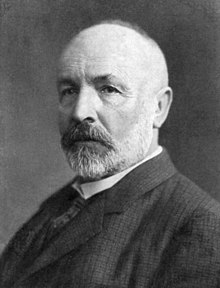
\includegraphics[width=0.4\textwidth]{01-figures/fig01.jpg}
    \caption{Picture of some guy}
    \label{fig:01}
\end{figure}

For the composition of tables, the font size should always be smaller than that of the rest of the text, and it is recommended to opt for the following format:

\begin{table}[H]
    \centering\small
    \begin{tabular}{@{}ccc@{}}
    \toprule
        \textbf{Formula} & \textbf{Test 1} & \textbf{Test 2} \\ 
    \midrule
        Compound 1 & $38.4$  &  $6.32$\\ 
        Compound 2 & $16.6$ & $12.5$ \\ 
    \bottomrule
    \end{tabular}
    \caption{Results from different substances.}
    \label{tab:01}
\end{table}

Tables, like figures, must always have a caption. This approach uses the \texttt{booktabs} package, which improves their presentation. You can also include code, such as the one shown in Code \ref{lst:01}.



% `lstlisting` comes from listing package and is used to include source code.
% Caption description called `listingname` (currently set to 'Code block') is configurable in format.text where listing package is imported

\begin{lstlisting}[language=Python,caption={Example of code},label={lst:01},captionpos=b]
# Bubble sort 
def BubbleSort(a):
    for i in range(len(a)-2):
        for j in range(len(a)-i-1):
            if a[j] > a[j+1]:
                a[j],a[j+1] = a[j+1],a[j]
    print("The list has been sorted.")
    return a
\end{lstlisting}

%%%%%%%%%%%%%%%%%%%%%%%%%%%%%%%%%%%%%%%%
\section{Conclusions}
%%%%%%%%%%%%%%%%%%%%%%%%%%%%%%%%%%%%%%%%

\begin{itemize}[leftmargin=*]
\item 
    Lorem ipsum dolor sit amet, consectetuer adipiscing elit. Ut purus elit, vestibulum ut, placerat ac, adipiscing vitae, felis. Curabitur dictum gravida mauris. Namarcu libero, nonummy eget, consectetuer id, vulputate a, magna. 
    Donec vehicula augue eu neque. Pellentesque habitant morbi tristique senectus et netus et malesuada fames ac turpis egestas. Mauris ut leo. Cras viverra metus rhoncus sem. Nulla et lectus vestibulum urna fringilla ultrices. Phasellus eu tellus sit amet tortor gravida placerat. Integer sapien est, iaculis in, pretium quis, viverra ac, nunc. Praesent eget sem vel leo ultrices bibendum. Aenean faucibus. Morbi dolor nulla, malesuada eu, pulvinar at, mollis ac, nulla. Curabitur auctor semper nulla. Donec varius orci eget risus. Duis nibh mi, congue eu, accumsan eleifend, sagittis quis, diam. Duis eget orci sit amet orci dignissim rutrum.

\item
    Nam dui ligula, fringilla a, euismod sodales, sollicitudin vel, wisi. Morbi auctor lorem non justo. Nam lacus libero, pretium at, lobortis vitae, ultricies et, tellus. Donec aliquet, tortor sed accumsan bibendum, erat ligula aliquet magna, vitae ornare odio metus a mi. Morbi ac orci et nisl hendrerit mollis. Suspendisse ut massa. Cras nec ante. Pellentesque a nulla. Cum sociis natoque penatibus et magnis dis parturient montes, nascetur ridiculus mus. Aliquam tincidunt urna. Nulla ullamcorper vestibulum turpis. Pellentesque cursus luctus mauris
\end{itemize}


%%%%%%%%%%%%%%%%%%%%%%%%%%%%%%%%%%%%%%%%

\section{Bibliography \& citations}

The bibliography must be included using a \(\texttt{.bib}\) file. The bibliography style to use is APA 7th edition. For citations, you can use the following commands as appropriate:

\begin{itemize}
\item 
    Full citation in parentheses \verb"\parencite{ }": \parencite{stewartpre}
\item
    Full citation with year in parentheses \verb"\textcite{ }": \textcite{stewartpre}
\item 
    Full citation without parenthese \verb"\cite{ }": \cite{stewartpre}
\item
    Cite author \verb"\citeauthor{ }": \citeauthor{stewartpre}
\item
    Cite year \verb"\citeyear{ }": \citeyear{stewartpre}
\item 
    Cite with extra options \verb"\parencite[ ][ ]{ }": \parencite[ver][p. 66]{stewartpre}
\end{itemize}

Note:  Citation handle (in this case \verb"stewartpre") is defined in \verb".bib" file.

%%%%%%%%%%%%%%%%%%%%%%%%%%%%%%%%%%%%%%%%

\subsection{Citation examples}


Apparently, only the first paragraph in a subsection in un-indented; all the rest are.
Según \textcite{stewartpre}, ``la forma más importante de visualizar una función es por medio de su gráfica'' (p. 152). Además, sabemos que ``la gráfica de una función $f$ da un retrato del comportamiento'' \parencite[p. 153]{stewartpre}. Por otro lado, una función se dice lineal porque su gráfica representa una recta \parencite{stewartpre}. Finalmente, según \textcite{stewartpre}:
\begin{quote}
    Por lo general consideramos funciones para las cuales los conjuntos $A$ y $B$ son conjuntos de números reales. El símbolo $f(x)$ se lee “$f$ de $x$” o “$f$ en $x$” y se denomina valor de $f$ en $x$, o la imagen de $x$ bajo $f$. El conjunto $A$ recibe el nombre de dominio de la función. El rango de $f$ es el conjunto de todos los valores posibles de $f(x)$ cuando $x$ varía en todo el dominio. (p. 125)
\end{quote}

This paragraph will be indented because it is not the first paragh of a subsection.
\begin{quote}
    Por lo general consideramos funciones para las cuales los conjuntos $A$ y $B$ son conjuntos de números reales. El símbolo $f(x)$ se lee “$f$ de $x$” o “$f$ en $x$” y se denomina valor de $f$ en $x$, o la imagen de $x$ bajo $f$. El conjunto $A$ recibe el nombre de dominio de la función. El rango de $f$ es el conjunto de todos los valores posibles de $f(x)$ cuando $x$ varía en todo el dominio. \parencite[p. 125]{stewartpre}
\end{quote}


%%%%%%%%%%%%%%%%%%%%%%%%%%%%%%%%%%%%%%%%

% Include to cite every entry in .bib file even if not referenced
%\nocite{*}

% Prevent overfull \hbox error when printing bibiography
\emergencystretch=1em
\printbibliography

\end{document}

